
\section{Theory}
\vspace{-0.5cm}
\singlespacing

\indent If \textit{velocity} is the rate \& direction of an object's \textit{position} over a certain time interval, then \textit{acceleration} is the rate \& direction of an object's \textit{velocity} over a certain time interval. So long as an object's velocity is changing, it has acceleration.\par 


Velocity and acceleration are both \textit{vector} quantities, meaning both have vertical and horizontal components. The vertical component of an object's acceleration is impacted by the Earth's gravity. The acceleration due to gravity on Earth's surface has been measured to be \textit{$9.80\thinspace{m/s^2}$}. \par

\begin{figure}[h!]
    \centering
    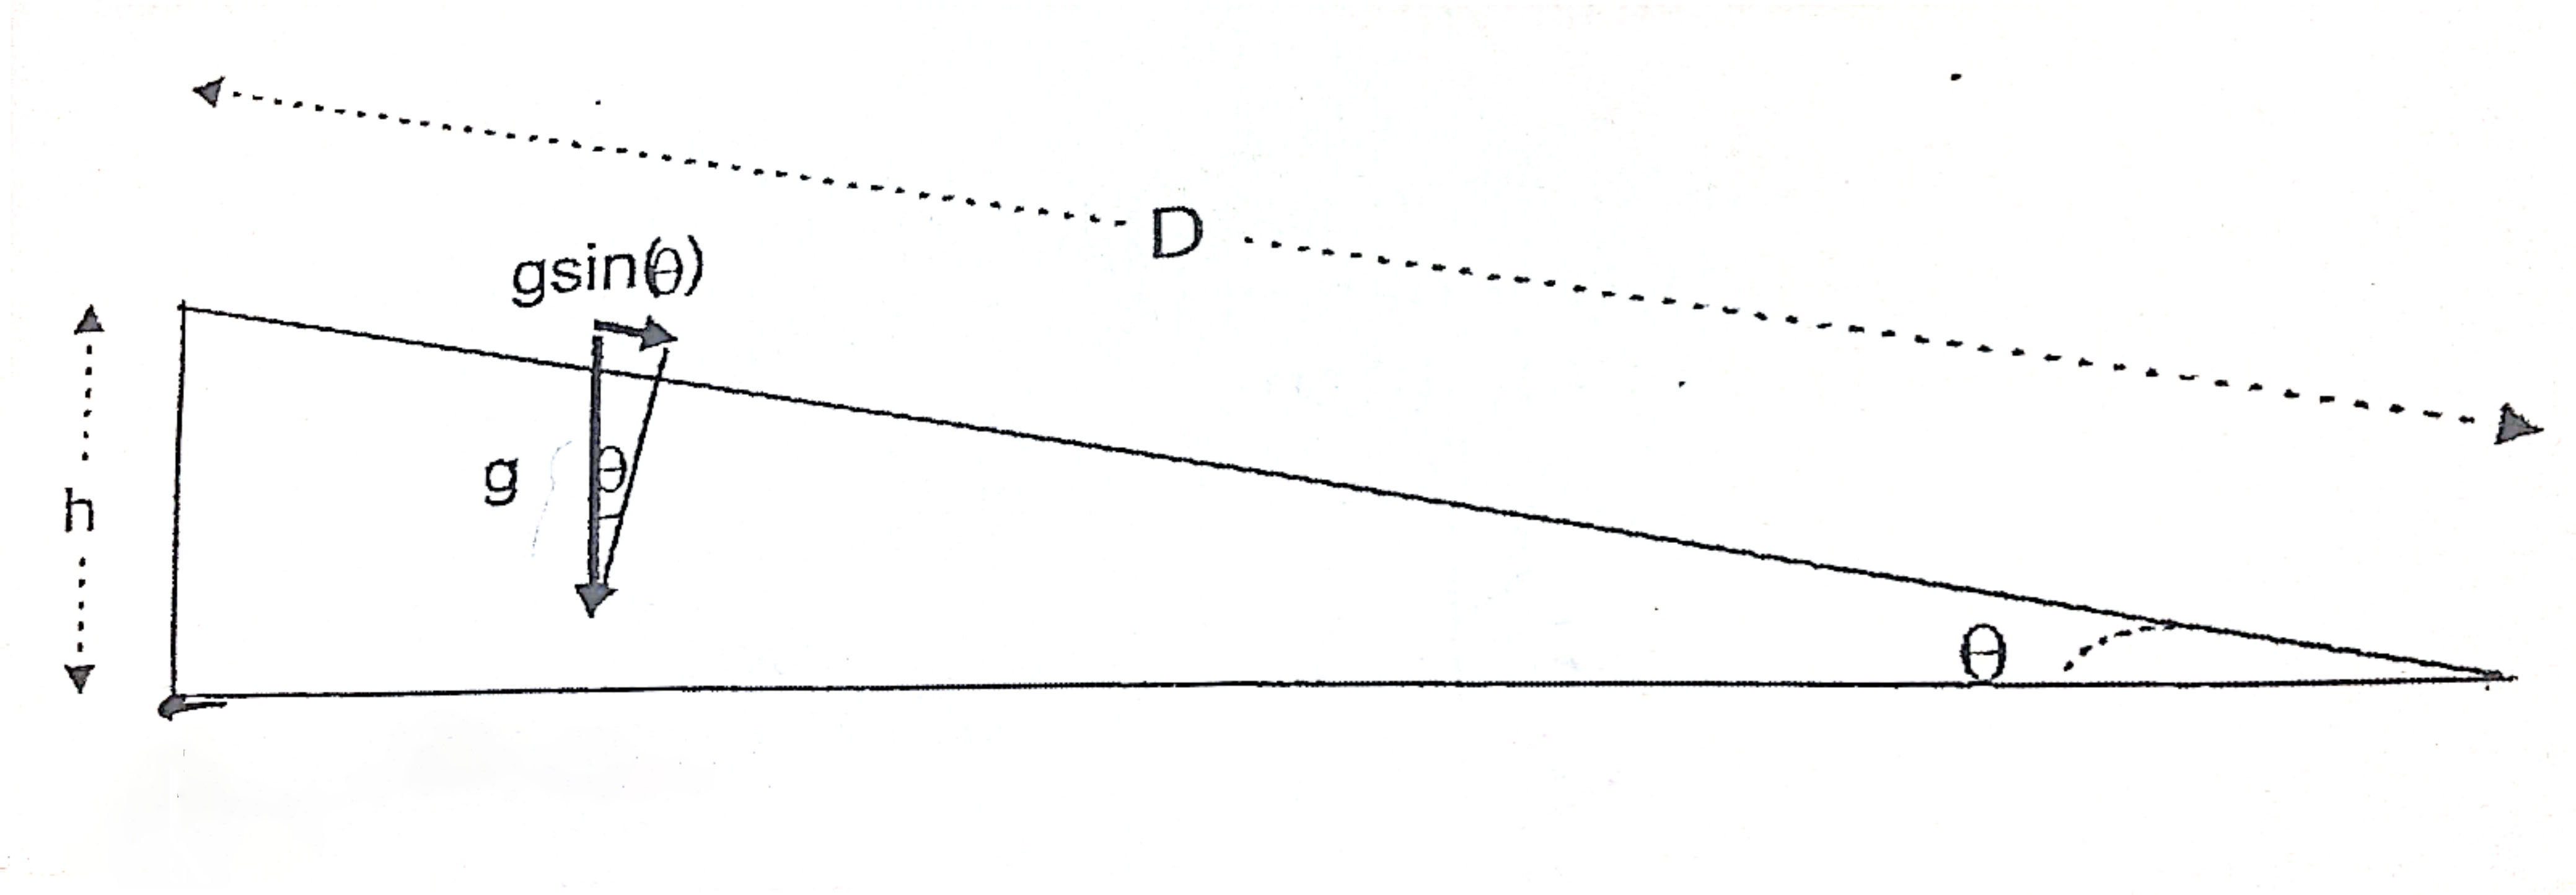
\includegraphics[width=0.8\textwidth]{figure1_inclineplane} % Example of adding a figure
    \caption{Incline plane}
    \label{fig:inclineplane}
\end{figure}

When objects fall straight down, assuming there's no air resistance, the vertical component of the object's acceleration is simply $9.80\thinspace{m/s^2}$. However, if the object is launched at an angle, then the object's acceleration in the vertical direction must be determined in a different way. Just as one would determine the horizontal \& vertical components of velocity for objects thrown at angles using trigonometric functions, so too can the acceleration due to gravity of such objects be calculated. More specifically, for objects that move along \textit{inclined planes} (see figure \ref{fig:inclineplane}), the component of the acceleration vector parallel to the plane can be calculated with the following equation:

\begin{equation}
a = gsin\theta
\label{eq:1}
\end{equation}

The plane angle (figure \ref{fig:inclineplane}) can be determined using:

\begin{equation}	
sin\theta = \frac{\Delta{h}}{D}
\label{eq:2}
\end{equation}

\newpage

